\section{Introduction}
\lipsum %delete this, just makes placeholder text.
Let's cite something in brackets \citep{Kearse2012geneious}. Let's cite two in brackets \citep{Kearse2012geneious, Belhaj2013}.

Let's add a figure of what the lac operon does because I have it to hand. See Figure \ref{fig:lacbanter}.
\begin{figure}[h]
    \centering
    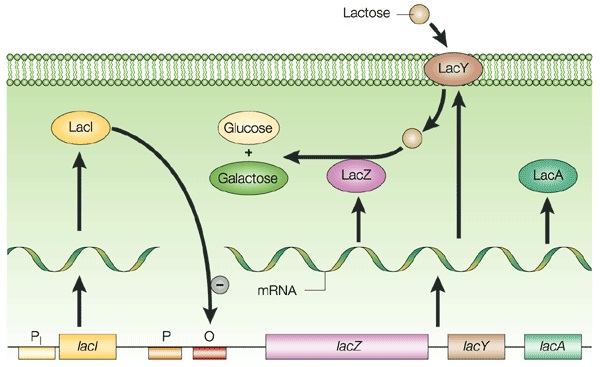
\includegraphics[width=0.6\textwidth]{lac.jpg}%width=1.0 is textwidth.
    \caption{Example figure.}
    \label{fig:lacbanter}%this is a unique identifier for this figure. Allows you to reference it in the text.
\end{figure}

Now let's insert a table, ya know, because we can. See Table \ref{tab:spam}.

\begin{table}[h]
\centering
\caption{Example table}
\label{tab:spam}
\begin{tabular}{|l|l|}
\hline
A thing & Another thing \\ \hline
Eggs    & 0             \\ \hline
SPAM    & 100+          \\ \hline
\end{tabular}
\end{table}
\section{Methods}
\lipsum %delete this, just makes placeholder text.
\newpage
\section{Results}
\lipsum %delete this, just makes placeholder text.
\newpage
\section{Discussion}
\lipsum %delete this, just makes placeholder text.
\newpage
\section{Main findings}
\lipsum %delete this, just makes placeholder text.